\documentclass[12pt]{article}

\usepackage[english]{babel}
\usepackage[utf8x]{inputenc}
\usepackage{amsmath}
\usepackage{graphicx}
\usepackage[colorinlistoftodos]{todonotes}
\usepackage{listings}
\usepackage{glossaries}
\usepackage{placeins}
\usepackage{fixltx2e}
\usepackage{pdfpages}
\usepackage{lastpage}
\usepackage{enumitem}
\usepackage{xcolor}
\usepackage{scrpage2}
\usepackage{scrtime}
\usepackage{parskip}
\usepackage{hyperref} 

\clearscrheadfoot
\pagestyle{scrheadings}
\usepackage[
top    = 2.5cm,
bottom = 3cm,
left   = 3cm,
right  = 3cm]{geometry}
\setcounter{secnumdepth}{4}
\title{Diploma Thesis}


\author{RoboNav}
\date{\today}


%Includes
\setlength{\parindent}{0cm}

\newcommand{\executeiffilenewer}[3]{%
\ifnum\pdfstrcmp{\pdffilemoddate{#1}}%
{\pdffilemoddate{#2}}>0%
{\immediate\write18{#3}}\fi%
}
\newcommand{\includesvg}[1]{%
\executeiffilenewer{#1.svg}{#1.pdf}%
{inkscape -z -D --file=#1.svg --export-pdf=#1.pdf --export-latex}%
\input{#1.pdf_tex}[width=1.0\textwidth]%
}

%Bibtex
\def\BibTeX{{\rm B\kern-.05em{\sc i\kern-.025em b}\kern-.08em
		T\kern-.1667em\lower.7ex\hbox{E}\kern-.125emX}}

%lslisting
\lstdefinestyle{customjava}{
  	language=Java,
  	frame=tlrb,
  	aboveskip=3mm,
  	belowskip=6mm,
  	showstringspaces=false,
  	columns=flexible,
  	basicstyle={\small\ttfamily},
  	numbers=none,
  	numberstyle=\tiny\color{gray},
  	keywordstyle=\color{purple},
  	commentstyle=\color{orange},
  	stringstyle=\color{blue},
  	breaklines=true,
  	breakatwhitespace=true
  	tabsize=3,
}

\lstset{escapechar=@,style=customjava}

%Cite right
\newcommand{\citeof}[2]{{
		\par \begingroup \leftskip=1cm \noindent \textit 
		''#1'' \cite{#2} \\
		\par \endgroup
	}}
	
% Picture insert (UseCase)
% \insertpicture{mik.png}{Some picture}{\cite{bk_key}}{itm:pic1}{0.5}
\newcommand{\insertpicture}[5]{{
	\begin{figure}[!htb]
		\centering\includegraphics[width=#5\textwidth]{#1}
		\caption[#2 #3]{#2}
		\label{#4}
	\end{figure}
	\FloatBarrier
}}
\makeglossaries
\newglossaryentry{json} {name=JSON, description={Java Script Object Notation}}
\newglossaryentry{GPS} {name=GPS, description={Global Positioning System }}
\newglossaryentry{NDGPS} {name=NDGPS, description={National Differential Global Positioning System }}
\newglossaryentry{WADGPS} {name=WADGPS, description={Wide Area Differential Global Positioning System }}
\newglossaryentry{QR} {name=QR, description={Quick Response (Code) }}
\newglossaryentry{RNCP} {name=RNCP, description={RoboNav Communication Protocol}}
\newglossaryentry{TGM} {name=TGM, description={Technologisches Gewerbe Museum / Institute of technology}}
\newglossaryentry{API} {name=API, description={Application Programming Interface}}
\newglossaryentry{JNI} {name=JNI, description={Java Native Interface}}
\newglossaryentry{WiFi} {name=WiFi, description={Wireless Local Area Network}}
\newglossaryentry{DHCP} {name=DHCP, description={Dynamic Host Configuration Protocol}}
\newglossaryentry{IP} {name=IP, description={Internet Protocol}}
\newglossaryentry{MOV} {name=MOV, description={QuickTime Movie (file extension)}}
\newglossaryentry{MPEG4} {name=MPEG4, description={Moving Picture Experts Group 4 (file extension)}}
\newglossaryentry{MJPEG} {name=MJPEG, description={Motion Joint Photographic Experts Group (file extension)}}
\newglossaryentry{JPEG} {name=JPEG, description={Joint Photographic Experts Group (file extension)}}
\newglossaryentry{CPU} {name=CPU, description={Central Processing Unit}}
\newglossaryentry{GHz} {name=GHz, description={Gigahertz (thousands of MHz)}}
\newglossaryentry{ROS} {name=ROS, description={Robot Operationg System}}
\newglossaryentry{GNUGPL} {name=GNU GPL, description={Gnu's Not Unix General Public License}}
\newglossaryentry{BSD} {name=BSD, description={Berkeley Software Distribution}}
\newglossaryentry{GUI} {name=GUI, description={Graphical User Interface}}
\newglossaryentry{DFT} {name=DFT, description={Discrete Fourier Transform}}
\newglossaryentry{RGB} {name=RGB, description={Red Green Blue}}
\newglossaryentry{UML} {name=UML, description={Unified Modeling Language}}
\newglossaryentry{MRDS} {name=MRDS, description={Microsoft Robotics Developer Studio}}
\newglossaryentry{IDE} {name=IDE, description={Integrated Development Environment}}
\newglossaryentry{FXML} {name=FXML, description={JavaFX - Extensible Markup Language file}}
\newglossaryentry{XML} {name=XML, description={Extensible Markup Language}}
\newglossaryentry{MVC} {name=MVC, description={Model View Control}}
\newglossaryentry{CSS} {name=CSS, description={Cascading Style Sheet}}

\renewcommand*\glspostdescription{\dotfill}




\begin{document}


\begin{titlepage}
\begin{center}

% Additional to first page

\includegraphics[width=0.7\textwidth]{images/logo}\\

\LARGE TGM - HTBLuVA Wien XX \\ IT Abteilung  \\[1.5cm]

% Title
\rule{1.0\textwidth}{1mm}
{ \huge \bfseries \\[0.4cm]  \huge Diplomarbeit \\ \LARGE Urban Green \\[0.4cm] }
\rule{1.0\textwidth}{1mm}

{ \huge Ramin Bahadoorifar \\ Matthias Schwebler \\ Samuel Schober \\ Konrad Kelc \\[0.4cm] }



\noindent 


\vfill

% Bottom of the page
{\small Version: \today ~at  \thistime    }
\end{center}

%\end{center}
\end{titlepage}


%HEADER AND FOOTER
\pagenumbering{Roman}
\ohead{\headmark}
\ifoot{© RoboNav - 2014/15}
\ofoot{\pagemark}

\newpage %----------------------------------------------------------------------------------------------
{\small\color{white}.}
\vspace{-0.7cm}
\tableofcontents

\newpage %----------------------------------------------------------------------------------------------
% Affirmation
%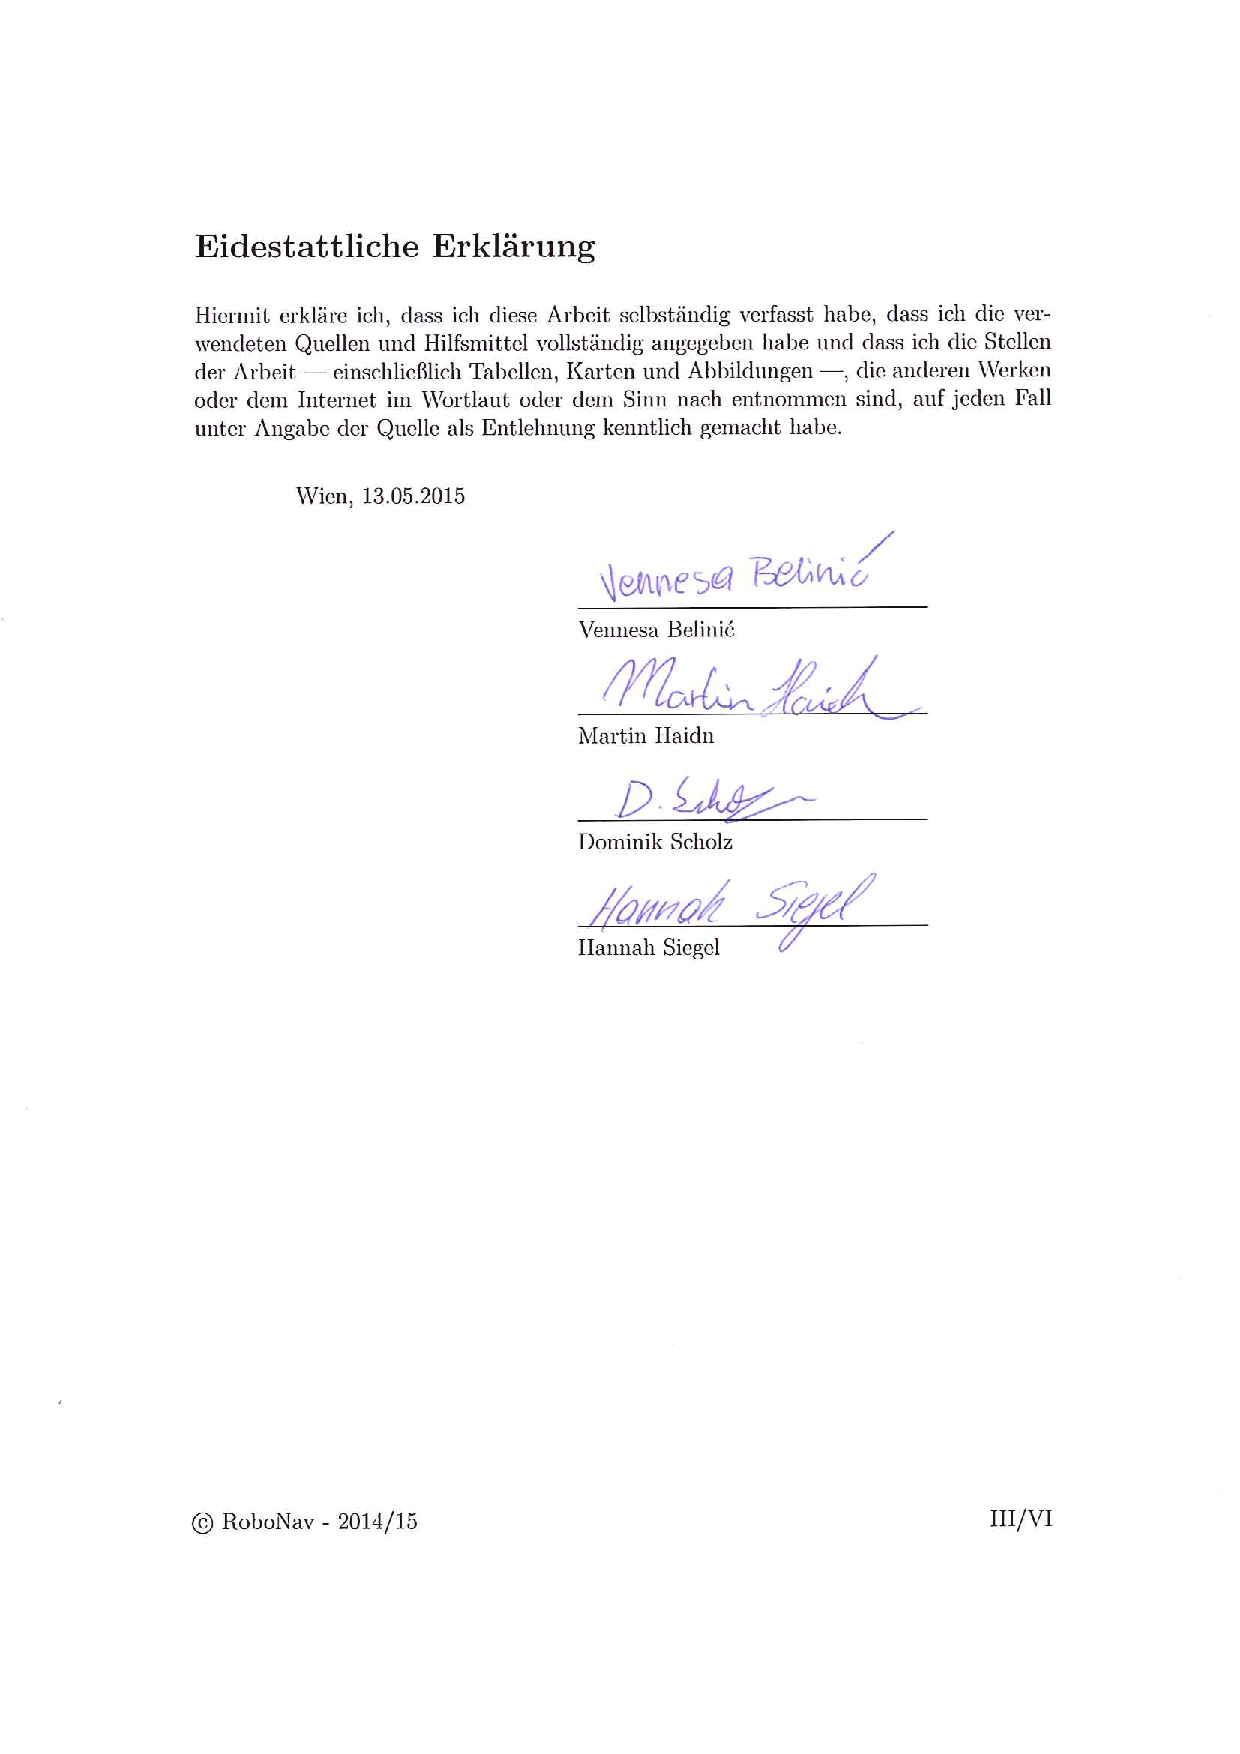
\includepdf[scale=1.2,pages=-]{documents/soor}
%\newpage
\section*{Abstract}
\cfoot{Matthias Schwebler}

*Abstract DE auf enlisch \"ubersetzen*

\newpage
\section*{Kurzfassung}
\cfoot{Matthias Schwebler}

Dieses Diplomprojekt, wird in Kooperation mit der Firma "Ponix Systems" durchgef\"uhrt und handelt \"uber die Entwicklung eines Low-Cost Prototypen eines Aquaponik Systems f\"ur den Heimgebrauch um dem globalen Trend der Umweltverbesserung zu folgen. Das Hauptziel unseres Projektes ist es, die derzeitige Marktl\"ucke von Aquaponik Systemen in Mitteleuropa zu f\"ullen. Daf\"ur wird ein pflegeleichtes \"Okosystem - bestehend aus einem Aquarium und einem Beet - entwickelt und auf die \"Uberwachung und Automatisierung optimiert. Dazu werden diverse Sensoren, Aktoren und Single Board Computer verbaut, welche die Regulierung der Parameter des Systems \"ubernehmen. Die Daten des Aquariums bzw. der Pflanzen werden an einen zentralen Server geleitet und dort persistiert um gegebenenfalls gew\"unschte Diagramme und Graphen zu erstellen. F\"ur die Persistierung wird auf Serverseite eine NoSQL Datenbank (MongoDB) verwendet und auf Seiten der Single Board Computer eine lightweight und schnelle (cache-artige) Datenbank verwendet (RedisDB).  Die Verbindung des \"Okosystems zum Internet wird von einem Single Board Computer \"ubernommen, der \"uber einen kleinen Touchscreen bedient werden kann. Selbst bei Internetunterbrechungen zeichnet das System weiterhin Daten auf und sendet sie bei erneutem Internetzugriff mit korrektem Zeitstempel an den Server.
\newpage
\section*{Acknowledgements}
\cfoot{}

We want to thank everyone. \\
 - Schabel (Idee, Grundstein) \\
 - Ponix Systems (Hardware, Softwareunterst\"utzung) \\
 - Koppensteiner (Bereitstellung des Arbeitsraums, Platz für Aquarium usw.) \\
TODO


\label{pageRomanEnd}

\newpage %----------------------------------------------------------------------------------------------
\pagenumbering{arabic}
\ofoot{\pagemark}

\section{Einf\"uhrung}
% Basic Introduction, Goal of the Project and very short description of the system (see section ...)
\label{sec:introduction}

\subsection{Einleitung}
%\input{}

\subsection{Aufgabenstellung}
%\input{}

\subsection{Ziele und Zielgruppen}
%\input{}

\subsection{Konzept}
%\input{}

\newpage %----------------------------------------------------------------------------------------------

\section{Grundlagen und vorhandene Technologien}
%\input{}

\newpage %----------------------------------------------------------------------------------------------
\subsection{Methodiken zur Verbreitung}
%\input{}
\newpage

\subsubsection{Citizen Science}
%\input{}

\newpage
\subsubsection{Blidungssektor}
%\input{}

\subsection{Vorhandene Aquaponiksysteme}
%\input{}

\newpage
\subsubsection{Grove Ecosystem}
%\input{}

\subsubsection{EcoQube C}
%\input{}

\subsubsection{Ponix Systems}
%\input{}



\newpage %----------------------------------------------------------------------------------------------
\section{Projektmanagement}
%\input{}

\subsection{Projektmanagement Methode}
%\input{}

\subsection{Teamstruktur}
%\input{}

\subsection{Aufgabenteilung}
%\input{}

\subsection{Terminplanung}
%\input{}

\subsection{User Stories}
%\input{}

\subsection{Sprint Dokumentation}
%\input{}

\newpage %----------------------------------------------------------------------------------------------
\section{Evaluierung der benötigten Technologien und Komponenten}
%\input{}

\subsection{Single Board Computer}
%\input{}

\subsection{Sensoren}
%\input{}

\subsection{Aktoren}
%\input{}

\subsection{Datenbankmanagementsystem}
%\input{}

\subsection{Webframework}
%\input{}

\subsection{Daten\"ubertragung}
%\input{}

\newpage %----------------------------------------------------------------------------------------------
\section{Projekt Umsetzung - Designunterlagen}
%\input{}

\subsection{Use-Case Diagramm}
%\input{}

\subsection{Datenakquisition}
%\input{}

\subsubsection{Technologie}
%\input{}

\subsubsection{Ablauf}
%\input{}

\subsection{Datenverarbeitung}
%\input{}

\subsubsection{Technologie}
%\input{}

\subsubsection{Umsetzung des Ablaufs}
%\input{}


\newpage %----------------------------------------------------------------------------------------------
\section{Zugriff auf das Aquaponik Systems}
%\input{}

\subsection{Userinterface - Frontend}
\subsubsection{User Experience}
\subsubsection{Browserkompatibilität}
\subsubsection{Technologien}
\subsubsection{Funktionen}
\subsubsection{Optimierungen}
\subsection{Zentralserver}
\subsubsection{Authentifikation}
\subsubsection{Kommunikation}
%\input{}

\newpage %----------------------------------------------------------------------------------------------
\section{Ausfallsicherheit und Konsistenzsicherung der Daten}
%\input{}

\subsection{Zwischenspeicherung beim Aquaponik System}
%\input{}

\subsubsection{Ausfall der Internetverbindung}
%\input{}

\subsubsection{Ausfall der Stromversorgung}
%\input{}

\newpage %----------------------------------------------------------------------------------------------
\section{Prototyp testing}
\subsection{Hardware}
\subsection{Prototyp}
\subsection{Aussichten}
%\input{}

\newpage %----------------------------------------------------------------------------------------------
\section{Ausblick}
%\input{}

\newpage %----------------------------------------------------------------------------------------------
\cfoot{}
\pagenumbering{roman}
\section{Appendix}
\label{sec:appenix}

\subsection{Glossaries}
\label{subsec:glossaries}
\begingroup
\renewcommand{\section}[2]{}
\printglossary[style=tree]
\endgroup
\newpage

{\small\color{white}.}
\vspace{-2cm}
\subsection{Figures}
\label{subsec:figures}
\begingroup
\renewcommand{\section}[2]{}
\listoffigures
\endgroup

\subsection{Listings}
\label{subsec:listings}
\begingroup
\renewcommand{\section}[2]{}
\lstlistoflistings
\endgroup

\subsection{Sources}
\label{subsec:sources}
\begingroup
\renewcommand{\section}[2]{}
\bibliographystyle{alpha}
\bibliography{sources}
\endgroup


\end{document}
